%!TEX root = ../../thesis_master.tex

%%%%%%%%%%
\chapter{Software Requirements Specification and Structured Analysis}
\label{chap:srs-sa}
%%%%%%%%%%

This chapter deals with the \emph{Software Requirement Specification} (SRS) \cite{IEEE8301998} and the \emph{Structured Analysis} \cite{SA_Braune} of the system developed in this work. Thanks to these two procedures, the objectives that the system must fulfill and a decomposition of it into different functions are stated. This leads to a complete definition of the system.

\nomenclature[ba]{SRS}{Software Requirement Specification}

The purpose of this work is to design a visual controller to provide an aerial robot the commands necessary to reach a desired pose with respect to a target object.

The visual servo controller developed is to be integrated into the \emph{Flypulator} aerial manipulator, a fully-actuated aerial robot equipped with a monocular monochrome camera pointing downwards. Since it is not available for testing during the development of this work, the \emph{hector\_quadrotor}\footnote{\url{http://wiki.ros.org/hector_quadrotor}} (see \cite{2012simpar_meyer}), an under-actuated aerial robot also equipped with a monocular monochrome camera pointing downwards, will be used.

%%%%%%%%%%
\section{Software Requirements Specification}
\label{sec:srs}
%%%%%%%%%%

In this section, the Software Requirement Specification \cite{IEEE8301998} for the visual servo controller developed in this thesis is presented. The use of SRS helps to define the system that is being designed, tracking continuously that the product developed satisfies the needs of the user. Only when every requirement stated therein is fulfilled the implementation would be completed.

%%%%%%%%%%
\subsection{Product Perspective}
\label{sec:product-perspective}
%%%%%%%%%%

The VS controller is to be used with an aerial robotic system based on the ROS framework. From the perspective of the robotic system, the VS controller will appear as a ROS node which publishes control commands through a ROS topic to the rest of the system.

The robotic system to be used with the controller is an aerial manipulator whose goal is to acquire a certain pose with respect to a target laying on the ground. 

The system developed here is to interact with the camera hardware of the robot, a monocular monochrome camera pointing downwards. The output of the system are the control inputs of the aerial robot system, a kinematic control is adopted, being these inputs the linear and angular velocities of the vehicle. These inputs interact with the already implemented inner control loop for the attitude of the robotic system and are the main input for the outer control loop, the one in charge of the translation.

% TODO: Add table with the hardware.

% TODO: State more accurately the how the inner and outer control loops interact with the attitude and position control.

% TODO : Sketch with the different control loops.

With the help of the visual servo controller, the robot is able to achieve a desired pose with respect to a target using only the visual information provided by the camera, so no pose computation is involved.

%%%%%%%%%%
\subsection{User Characteristics}
\label{sec:user-characteristics}
%%%%%%%%%%

The product developed in this thesis will be used as part of a ROS-based system, thus the expected user is a designer willing to implement an Image Based Visual Servoing control strategy for his/her robotic system. The user should be familiarized with the ROS framework and the system will need the structure and interfaces of any standard ROS product.

%%%%%%%%%%
\subsection{Assumptions and Dependencies}
\label{sec:assumptions-dependencies}
%%%%%%%%%%

The software  has been tested on the following platform. Forward or backward support is not guaranteed on a different set-up.

\begin{itemize}
	\item ROS version: ROS Indigo\footnote{\url{http://wiki.ros.org/indigo}}
	\item Operating System: Ubuntu 14.04\footnote{\url{http://releases.ubuntu.com/14.04/}} Trusty Tahr, 64 bit
\end{itemize}

%%%%%%%%%%
\subsection{Functional Requirements}
\label{sec:functional-requirements}
%%%%%%%%%%

The functional requirements describe what the system must do to complete the overall task:

\begin{itemize}
	\item \textbf{F1}: \emph{Compute desired visual features}. For the desired pose with respect to the target, compute a vector of image features. 
	
	\item \textbf{F2}: \emph{Compute current visual features}. For the current pose with respect to the target, compute a vector of image features from the target. 
	
	\item \textbf{F3}: \emph{Compute feature difference}. Compute the difference between the current feature vector and the desired feature vector to be used as error for the control law.		
	
	\item \textbf{F4}: \emph{Provide velocity commands to the low level controller}. Control input based on image data so that the aerial robot achieves the desired pose with respect to the target.Velocity control based on the error between current and desired image features, no pose estimation.
	
	\item \textbf{F5}: \emph{Provide feedback to the user and terminate the visual servoing task}. The system must be able to tell the user whether the target pose has been already achieved or not, by publishing the current error of the controller. Once the desired pose has been achieved, it must notify the user and disconnect from the robot.
\end{itemize}

%%%%%%%%%%
\subsection{Qualitative Requirements}
\label{sec:other-requirements}
%%%%%%%%%%

\begin{itemize}
	\item \textbf{A1}: All components are working reliably.
	\item \textbf{A2}: The software is sufficiently fast, modular and modifiable.
	\item \textbf{A3}: The implementation is transparent and comprehensible.
	\item \textbf{A4}: Control inputs must provide stable and smooth flight maneuvers.
	\item \textbf{A5}: Robot must be able to start from different initial positions.
	\item \textbf{A6}: Algorithm must be fast enough to allow real time control of the aerial robot.
	\item \textbf{A7}: The implementation should follow the style guide of ROS \cite{ROS_Style}.
\end{itemize}

%%%%%%%%%%
\subsection{General Constraints}
\label{sec:general-constraints}
%%%%%%%%%%

\begin{itemize}
	\item The environment must be sufficiently illuminated for the camera to work.
	\item The observed object must be planar and continuous and provided to the program as a binary image obtained by segmentation algorithms.
	\item The target pose must be provided by a sufficient number of features.
	\item The target must be always in the filed of view of the camera, so features can be extracted an control input computed.
	\item Testing computer is a MacBook Pro\footnote{\url{https://everymac.com/systems/apple/macbook_pro/specs/macbook-pro-core-i5-2.7-13-early-2015-retina-display-specs.html}} (Early 2015) with 2.7 GHz Intel Core i5 processor, 8 GB 1867 MHz DDR3 memory and Intel Iris Graphics 6100 1536 MB graphics. Linux OS is run using Oracle VM VirtualBox\footnote{\url{www.virtualbox.org}} (Version 5.1.14 r112924) with 5 GB base memory and two processors.
\end{itemize}

\nomenclature[ba]{OS}{Operative System}

\pagebreak

%%%%%%%%%%
\section{Structured Analysis}
\label{sec:sa}
%%%%%%%%%%

The \emph{Structured Analysis} \cite{Janschek2011} is a formal method to describe relationships of functional type in complex processes. In order to do that, it views the system from the perspective of data flowing through it. The Structured Analysis is a top-down model, meaning that it analyses the system data flows through successive decomposition. The result of the Structured Analysis of a system is a set graphical diagrams representing the different processes or functions applied to the data and the outputs stored by the system.

% TODO: Continue with next paragraph:

% In this work, the system has been divided in ... levels ...

%%%%%%%%%%
\subsection{Context Diagram}
\label{sec:context-diagram}
%%%%%%%%%%

The \emph{Context Diagram} shows the interfaces between the system developed in this work and its environment.

\begin{figure}[h]
	\caption{Context Diagram}
	\label{fig:sa_diag_01}
	\centering
	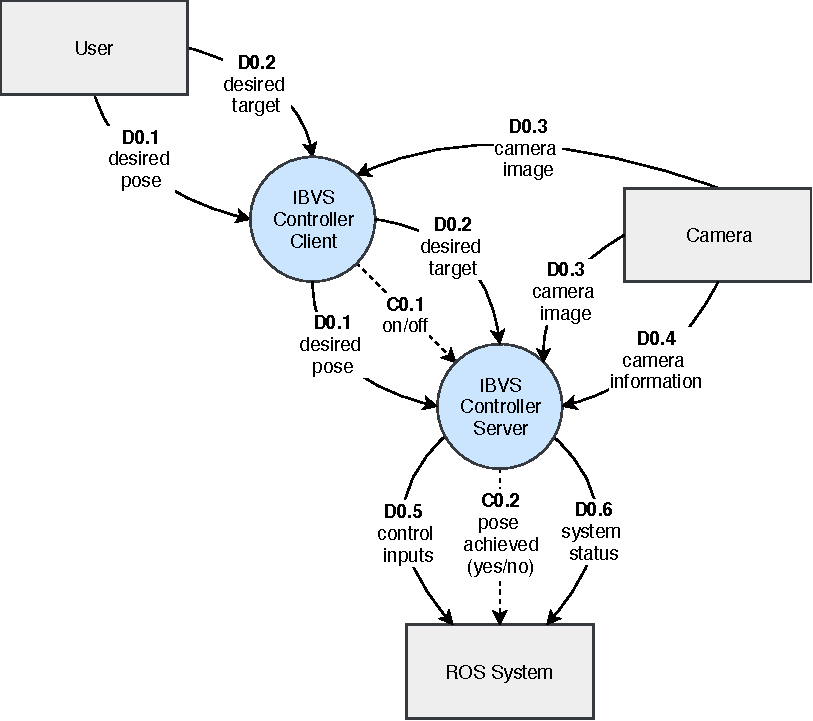
\includegraphics[width=0.8\textwidth]{content/chapter_03/images/sa_diagram_01.pdf}
\end{figure}

%%%%%%%%%%
\subsection{Level A: IBVS Controller}
\label{sec:level-A}
%%%%%%%%%%

Level A is the first level below the context diagram and contains the main functions (defined in Section \ref{sec:functional-requirements} as F1, F2, F3, F4 and F5) of the system developed, the \textit{IBVS Controller Server}. In Figure \ref{fig:sa_diag_02} a \emph{Data Flow Diagram} (DFD) is used to describe the interaction between data and processes. A Data Flow Diagram \cite{Janschek2011} is a decomposition of the system developed resultant of the subjective perspective of the design engineer about it.

\nomenclature[ba]{DFD}{Data Flow Diagram}
\nomenclature[ba]{DD}{Data Dictionary}

\begin{figure}[!htb]
	\caption{Data Flow Diagram - Level A}
	\label{fig:sa_diag_02}
	\centering
	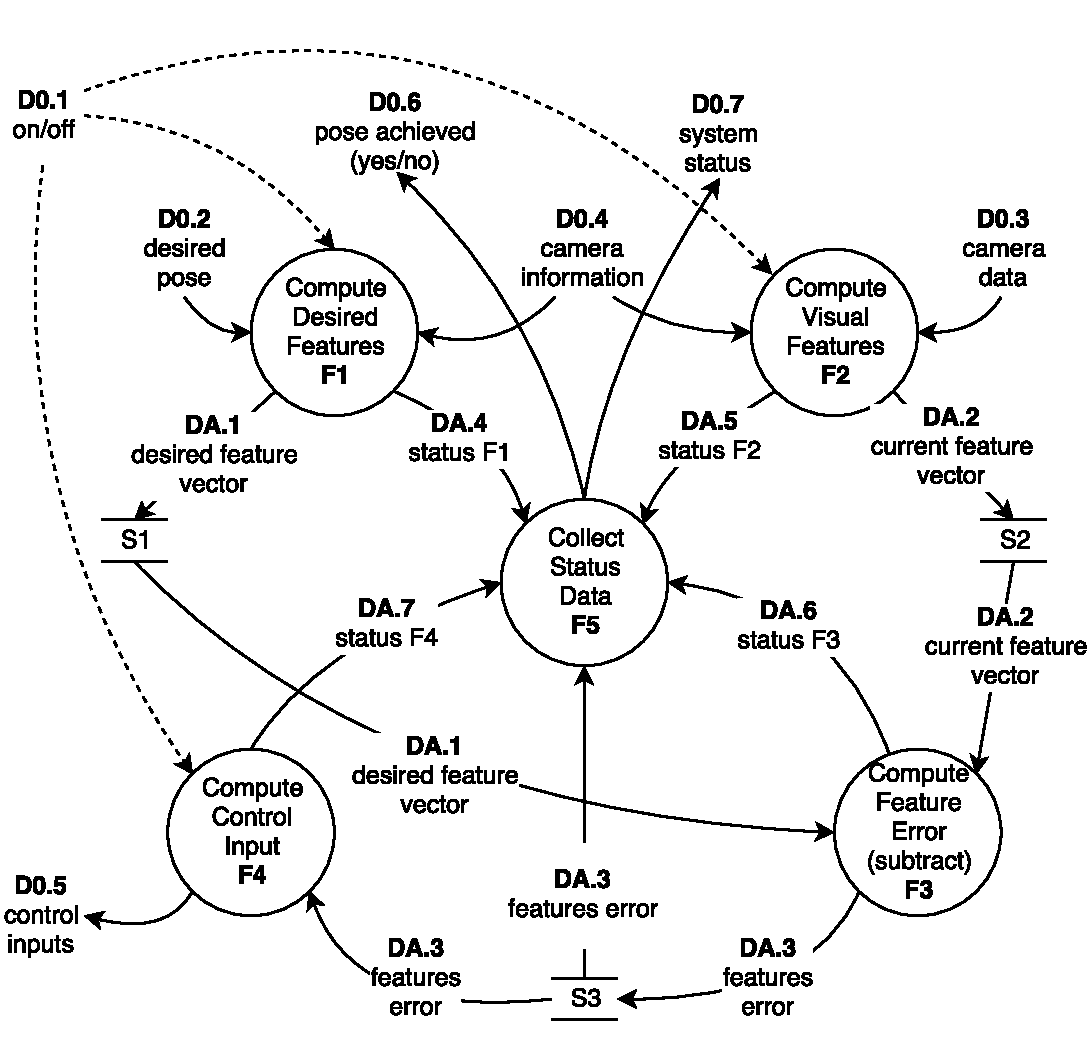
\includegraphics[width=\textwidth]{content/chapter_03/images/sa_diagram_02.pdf}
\end{figure}

\pagebreak

Table \ref{tab:DD-LA} contains the \emph{Data Dictionary} (DD) for the DFD of Level A. The Data Dictionary \cite{Janschek2011} is a detailed representation of all data flows involved in a Data Flow Diagram. Where $D = \text{data flow}$ and $C = \text{control flow}$.

\begin{table*}[!htb]
	\caption{Data Dictionary for Level A}
	\label{tab:DD-LA}
	\centering
	\begin{tabular}{lll}
		\toprule
		Flow & Type & Description \\
		\midrule
		C0.1 & C & User input to start or stop the system \\
		C0.2 & C & Information about pose achieved or not \\
		D0.1 & D & User defined desired target ID \\
		D0.2 & D & User defined desired camera pose w.r.t. the target \\
		D0.3 & D & Camera image data \\
		D0.4 & D & Camera information (sensor data, camera model, etc.) \\
		D0.5 & D & Velocity commands in the $E$ frame \\
		D0.6 & D & System status \\
		\midrule
		DA.1 & D & Feature vector for desired pose \\
		DA.2 & D & Feature vector from current camera image data \\
		DA.3 & D & Features difference vector used for control law \\
		DA.4 & D & System status from process F1 \\
		DA.5 & D & System status from process F2 \\
		DA.6 & D & System status from process F3 \\
		DA.7 & D & System status from process F4 \\
		\midrule
		S1 & Datastore & Desired feature vector \\
		S2 & Datastore & Current feature vector \\
		S3 & Datastore & Feature difference vector \\
		\bottomrule
	\end{tabular}
\end{table*}

\pagebreak

%%%%%%%%%%
\subsection{Level B1: Compute Desired Visual Features}
\label{sec:level-B1}
%%%%%%%%%%

% TODO: In case of design alternative, this level may change. Desing variants are named with letters.

Figure \ref{fig:sa_diag_03} contains the Data Flow Diagram that describes the inner work of the process \textit{F1: Compute desired visual features}.

\begin{figure}[!htb]
	\caption{Data Flow Diagram - Level B1}
	\label{fig:sa_diag_03}
	\centering
	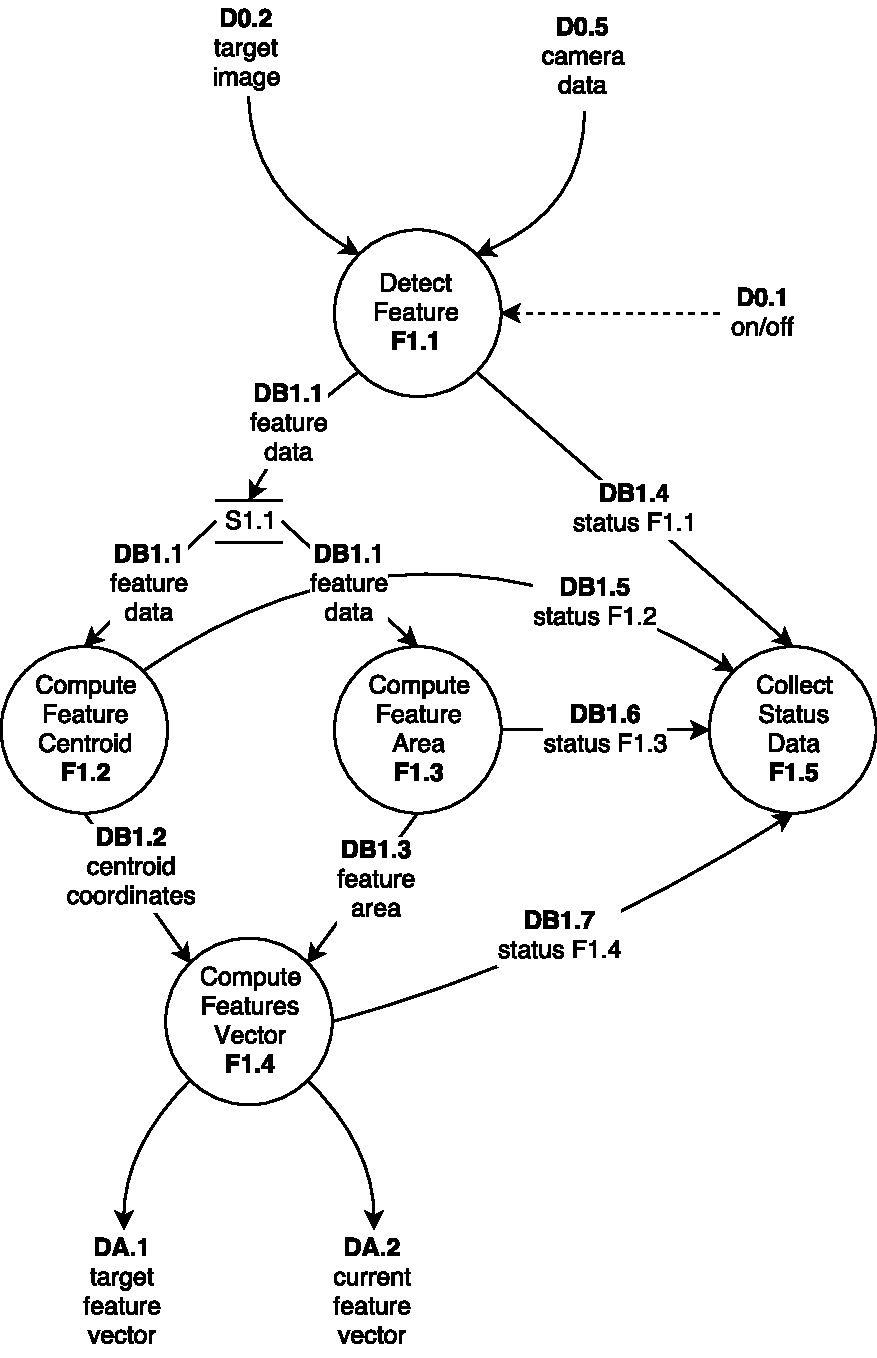
\includegraphics[width=0.8\textwidth]{content/chapter_03/images/sa_diagram_03.pdf}
\end{figure}

\pagebreak

%%%%%%%%%%
\subsection{Level B2: Compute Current Visual Features}
\label{sec:level-B2}
%%%%%%%%%%

Figure \ref{fig:sa_diag_04} contains the Data Flow Diagram that describes the inner work of the process \textit{F2: Compute current visual features}.

\begin{figure}[!htb]
	\caption{Data Flow Diagram - Level B2}
	\label{fig:sa_diag_04}
	\centering
	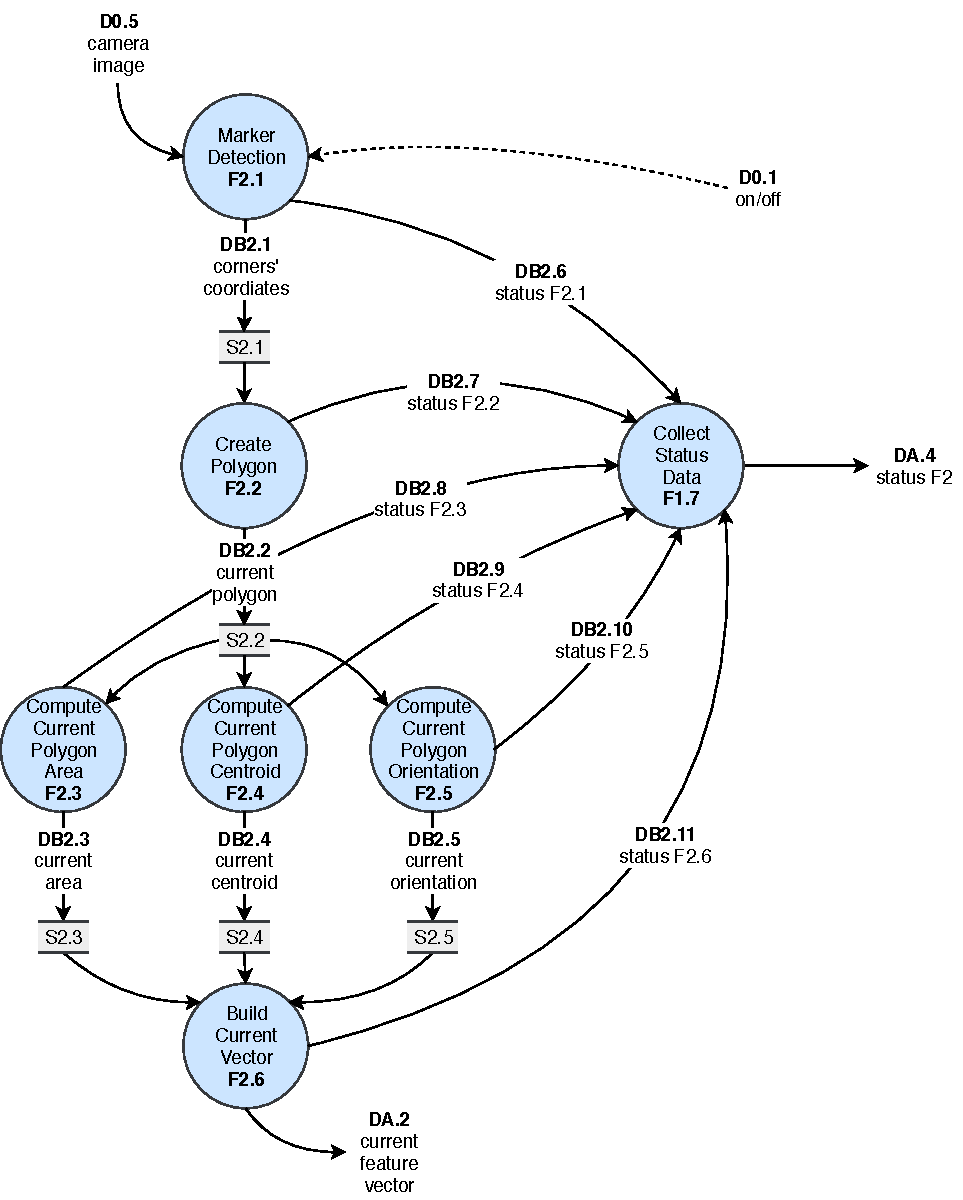
\includegraphics[width=0.8\textwidth]{content/chapter_03/images/sa_diagram_04.pdf}
\end{figure}

\pagebreak

%%%%%%%%%%
\subsection{Level B3: Compute Control Law}
\label{sec:level-B3}
%%%%%%%%%%

Figure \ref{fig:sa_diag_05} contains the Data Flow Diagram that describes the inner work of the process \textit{F4: Compute control law}.

\begin{figure}[!htb]
	\caption{Data Flow Diagram - Level B3}
	\label{fig:sa_diag_05}
	\centering
	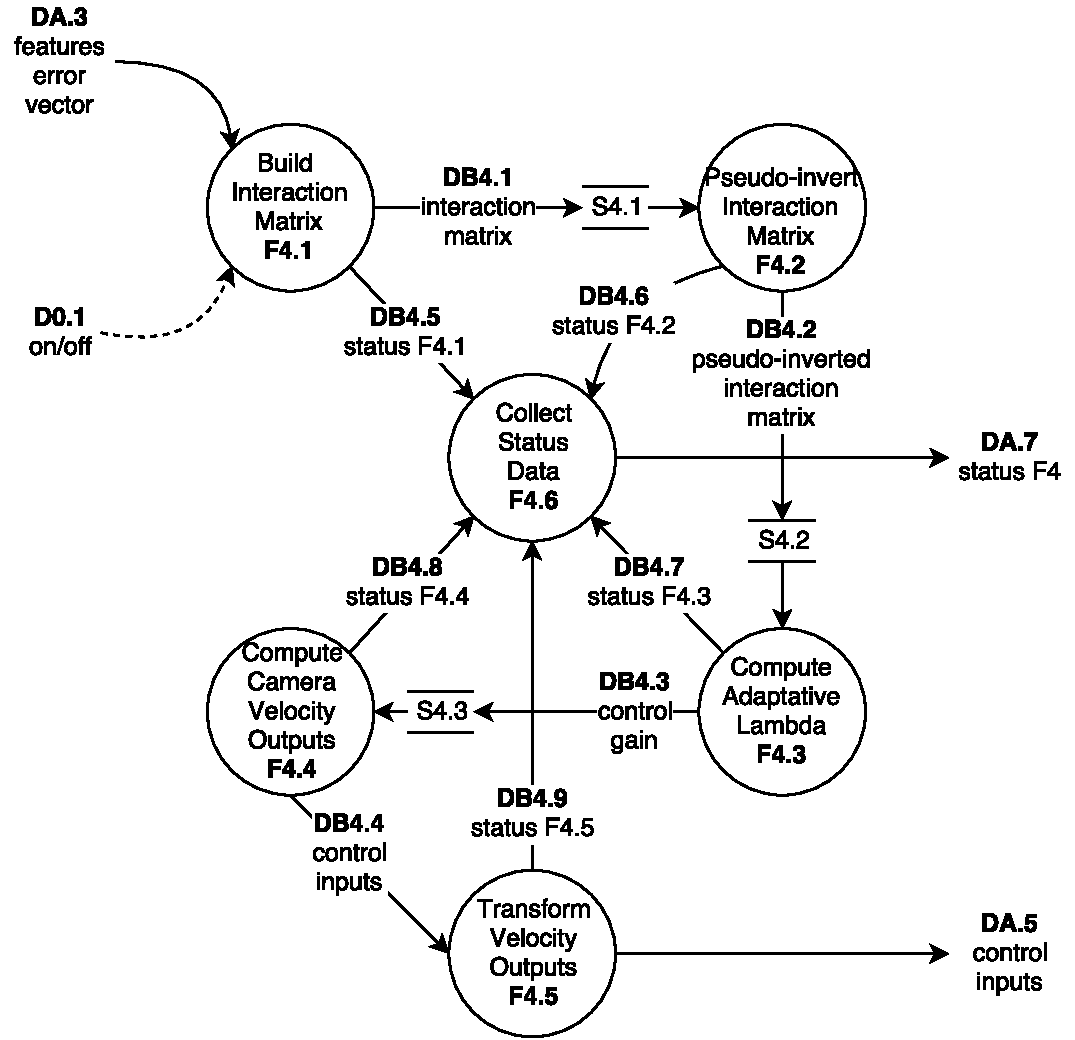
\includegraphics[width=\textwidth]{content/chapter_03/images/sa_diagram_05.pdf}
\end{figure}

\pagebreak

\begin{table*}[!htb]
	\caption{Data Dictionary for Level B}
	\label{tab:DD-LB-a}
	\centering
	\begin{tabular}{lll}
		\toprule
		Flow & Type & Description \\
		\midrule
		DB1.1 & D & Desired corners' coordinates in the image plane\\
		DB1.2 & D & Desired polygon object \\
		DB1.3 & D & Desired polygon area \\
		DB1.4 & D & Desired polygon centroid coordinates in the image plane \\
		DB1.5 & D & System status from process F1.1 \\
		DB1.6 & D & System status from process F1.2 \\
		DB1.7 & D & System status from process F1.3 \\
		DB1.8 & D & System status from process F1.4 \\
		DB1.9 & D & System status from process F1.5 \\
		\midrule
		DB2.1 & D & Marker corners' coordinates in the image plane \\
		DB2.2 & D & Current polygon object \\
		DB2.3 & D & Current area of the polygon \\
		DB3.4 & D & Current polygon centroid coordinates in the image plane \\
		DB2.5 & D & Current angle of orientation of the target \\
		DB2.6 & D & System status from process F2.1 \\
		DB2.7 & D & System status from process F2.2 \\
		DB2.8 & D & System status from process F2.3 \\
		DB2.9 & D & System status from process F2.4 \\
		DB2.10 & D & System status from process F2.5 \\
		DB2.11 & D & System status from process F2.6 \\
		\midrule
		DB4.1 & D & Visual servoing interaction matrix \\
		DB4.2 & D & Pseudo-inverted visual servoing interaction matrix \\
		DB4.3 & D & Control gain $\lambda$ \\
		DB4.4 & D & Velocity control inputs in camera frame \\
		DB4.5 & D & System status from process F4.1 \\
		DB4.6 & D & System status from process F4.2 \\
		DB4.7 & D & System status from process F4.3 \\
		DB4.8 & D & System status from process F4.4 \\
		DB4.9 & D & System status from process F4.5 \\
		\bottomrule
	\end{tabular}
\end{table*}

\begin{table*}[!h]
	\caption{Datastore Dictionary for Level B}
	\label{tab:DD-LB-b}
	\centering
	\begin{tabular}{lll}
		\toprule
		Flow & Type & Description \\
		\midrule
		S1.1 & Datastore & Target marker ID \\
		S1.2 & Datastore & geometry\_msgs/Pose of frame $C$ w.r.t. frame $O$ \\
		S1.3 & Datastore & Coordinates of the desired marker's corners in the image plane \\
		S1.4 & Datastore & Desired polygon object \\
		S1.5 & Datastore & Desired polygon area \\
		S1.6 & Datastore & Desired polygon centroid coordinates in the image plane \\
		S2.1 & Datastore & Marker corners' coordinates in the image plane \\
		S2.2 & Datastore & Current target polygon object  \\
		S2.3 & Datastore & Current polygon area \\
		S2.4 & Datastore & Current polygon centroid coordinates in the image plane \\
		S2.5 & Datastore & Current polygon orientation angle \\	
		S4.1 & Datastore & Visual servoing interaction matrix \\	
		S4.2 & Datastore & Pseudo-inverted Visual Servoing interaction matrix \\
		S4.3 & Datastore & Control gain $\lambda$ \\
		\bottomrule
	\end{tabular}
\end{table*}